\chapter{Eenvoudige Classifiers}
\begin{itemize}
	\item Typische voorbeelden van segmentatieproblemen:
	\begin{itemize}
		\item 
		Kunnen we de grijze waarden gebruiken om de pixels van een weg te onderscheiden van de omgevingspixels?
		
		\begin{figure}[ht]
			\centering
			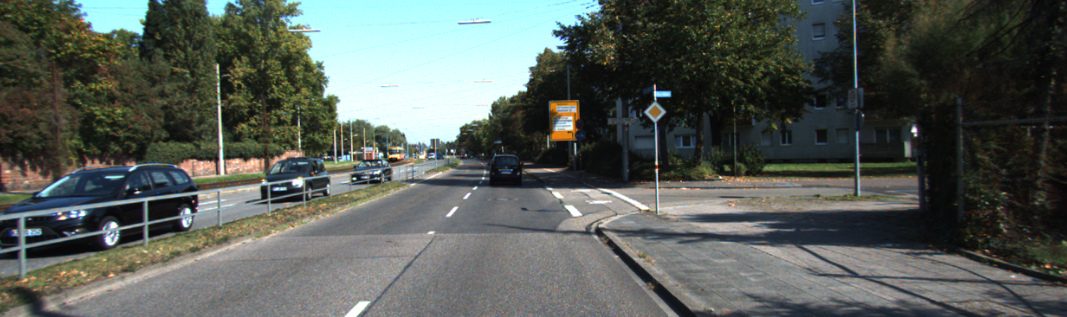
\includegraphics[width=0.5\linewidth]{segmentation_road}
			\caption{Een weg.}
			\label{fig:segmentation_road}
		\end{figure}
	
		\item 
		De kleur van de muur is lichter dan die van het schilderij. Kan de intensiteit van de kleur gebruikt worden om het schilderij te onderscheiden van de muur?
		
		\begin{figure}[ht]
			\centering
			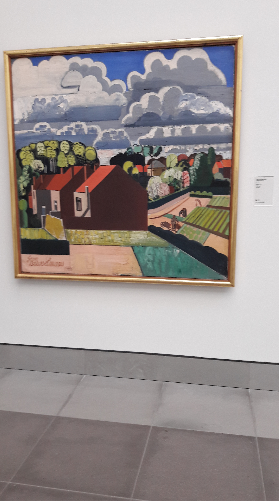
\includegraphics[width=0.25\linewidth]{segmentation_painting}
			\caption{Een schilderij.}
			\label{fig:segmentation_painting}
		\end{figure}
	\end{itemize}
\end{itemize}

\newpage
\section{Discriminerende classifiers}
\begin{figure}[ht]
	\centering
	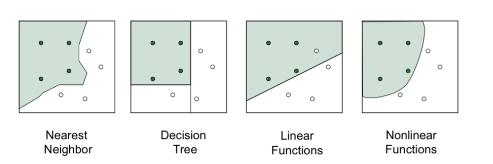
\includegraphics[width=\linewidth]{discriminant_classifiers}
\end{figure}
\begin{itemize}
	\item Dit zijn classifiers die hun classificatie enkel bepalen aan de hand van de training data.
	\item $g(\textbf{x}) = C_k$. Hierbij is $\textbf{x}$ de feature vector en $C_k$ de beschrijving van klasse $k$.
	\item $g(\textbf{x}) = 0$ is de \textbf{beslissingsrand} (in twee dimensies is dit een lijnstuk, in drie dimensies een vlak, ... Meer algemeen spreekt men van een hyperoppervlak.).
	\item Lineaire functie:
	$g(\textbf{x}) = \textbf{w}^T\textbf{x} + b = \begin{pmatrix}w_1 & ... & w_n\end{pmatrix}\begin{pmatrix}
	x_1 \\ ... \\ x_n
	\end{pmatrix} + b$ 
		\item Kwadratische functie:
	$g(\textbf{x}) = \textbf{w}^T\textbf{A}\textbf{x} + b =  \begin{pmatrix}w_1 & ... & w_n\end{pmatrix}
	\begin{pmatrix}
	h_{11} & ... & ... \\
	... & ... & ... \\
	... & ... & h_{nn}
	\end{pmatrix}
	\begin{pmatrix}
	x_1 \\ ... \\ x_n
	\end{pmatrix} + b$ 
	\item Hierbij is $\textbf{w}$ de gewichtenmatrix en $\textbf{A}$ een vierkantsmatrix met coëfficiënten.
\end{itemize}

\subsection{Pixel classificatie voor grijswaarden}
\begin{itemize}
	\item Als we figuur \ref{fig:segmentation_road} converteren  naar grijsschaal, dan kan een histogram van de grijswaarden bekomen worden (figuur \ref{fig:segmentation_road_histogram}).
	\begin{figure}[ht]
		\centering
		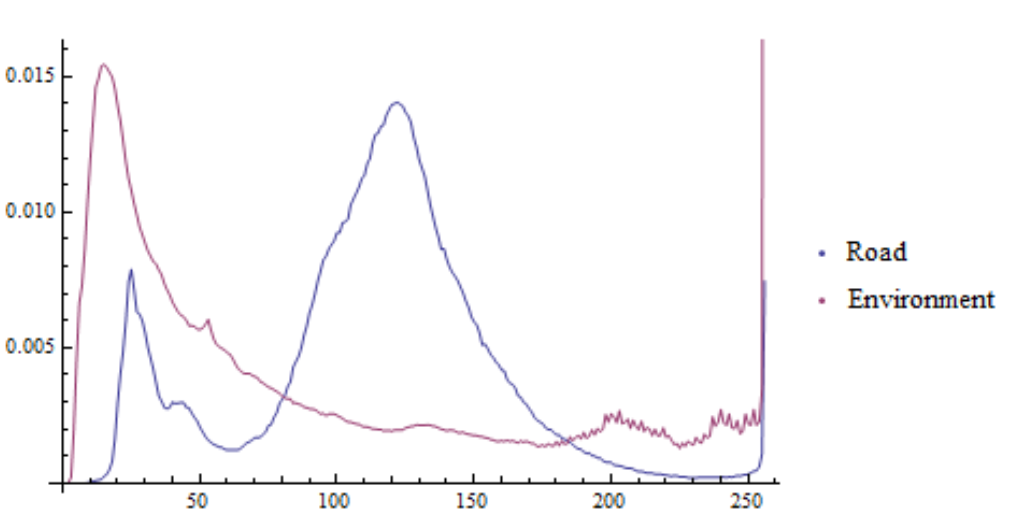
\includegraphics[width=\linewidth]{segmentation_road_histogram}
		\caption{Histogram van de grijswaarden voor zowel het wegdek als de omgeving.}
		\label{fig:segmentation_road_histogram}
	\end{figure}
	\item De x-as bevat de intensiteit van de grijswaarde (0 tot 255) en de y-as bevat de relatieve frequentie dat die grijswaarde voorkomt. 
	
	\item Zowel weg en omgeving krijgt een piek op 255. Dit komt omdat de camera satureert en er geen hogere waardere meer is.
	\item De functies overlappen dus er kan geen eenvoudige classifier gemaakt worden.
\end{itemize}
\subsection{Pixel classificatie voor kleurwaarden}
\begin{itemize}
	\item De kleurwaarden van figuur \ref{fig:segmentation_road} kan ook visueel voorgesteld worden voor zowel het wegdek als de omgeving (figuur \ref{fig:rgb_road} en \ref{fig:rgb_nonroad})
	\begin{figure}[!htb]
		\begin{minipage}{0.48\textwidth}
			\centering
			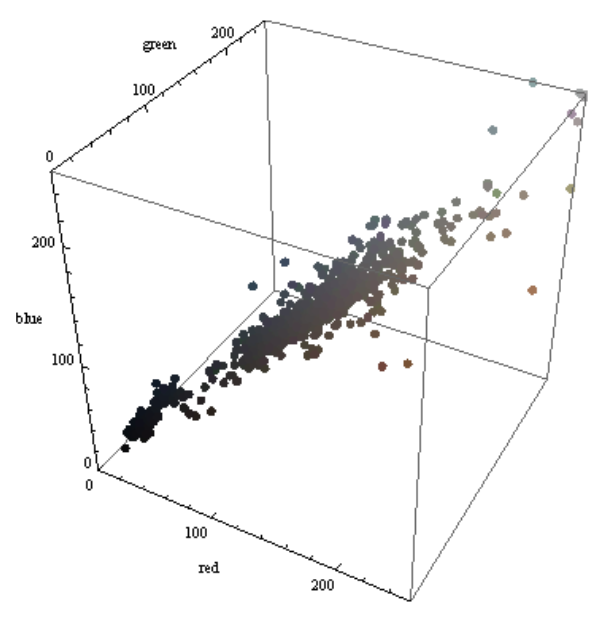
\includegraphics[width=0.9\linewidth]{road_color}
			\caption{RGB waarden van het wegdek.}
			\label{fig:rgb_road}
		\end{minipage}\hfill
		\begin{minipage}{0.48\textwidth}
			\centering
			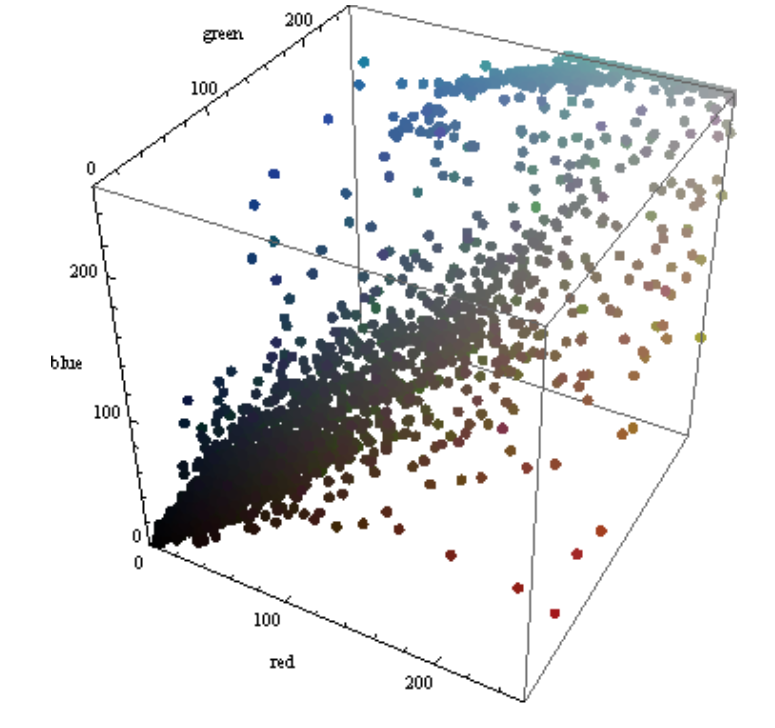
\includegraphics[width=0.9\linewidth]{nonroad_color}
			\caption{RGB waarden van de omgeving.}
			\label{fig:rgb_nonroad}
		\end{minipage}
	\label{epic}
	\end{figure}


\end{itemize}